\chapter{図・表・数式・コードの記法}
\label{chap:float}

本章では，論文で多用する図・表・数式・ソースコードについて，
さまざまな記法のパターンを丁寧に示す．

%% ===========================================================
\section{図の基本}
\label{sec:figure}
図は\texttt{figure}環境に入れる．\verb|\centering|で中央寄せし，
キャプションは\verb|\caption{}|で図の下に付け，\verb|\label{}|で参照できるようにする（図\ref{fig:basic}）．

\begin{figure}[htbp]
    \centering
    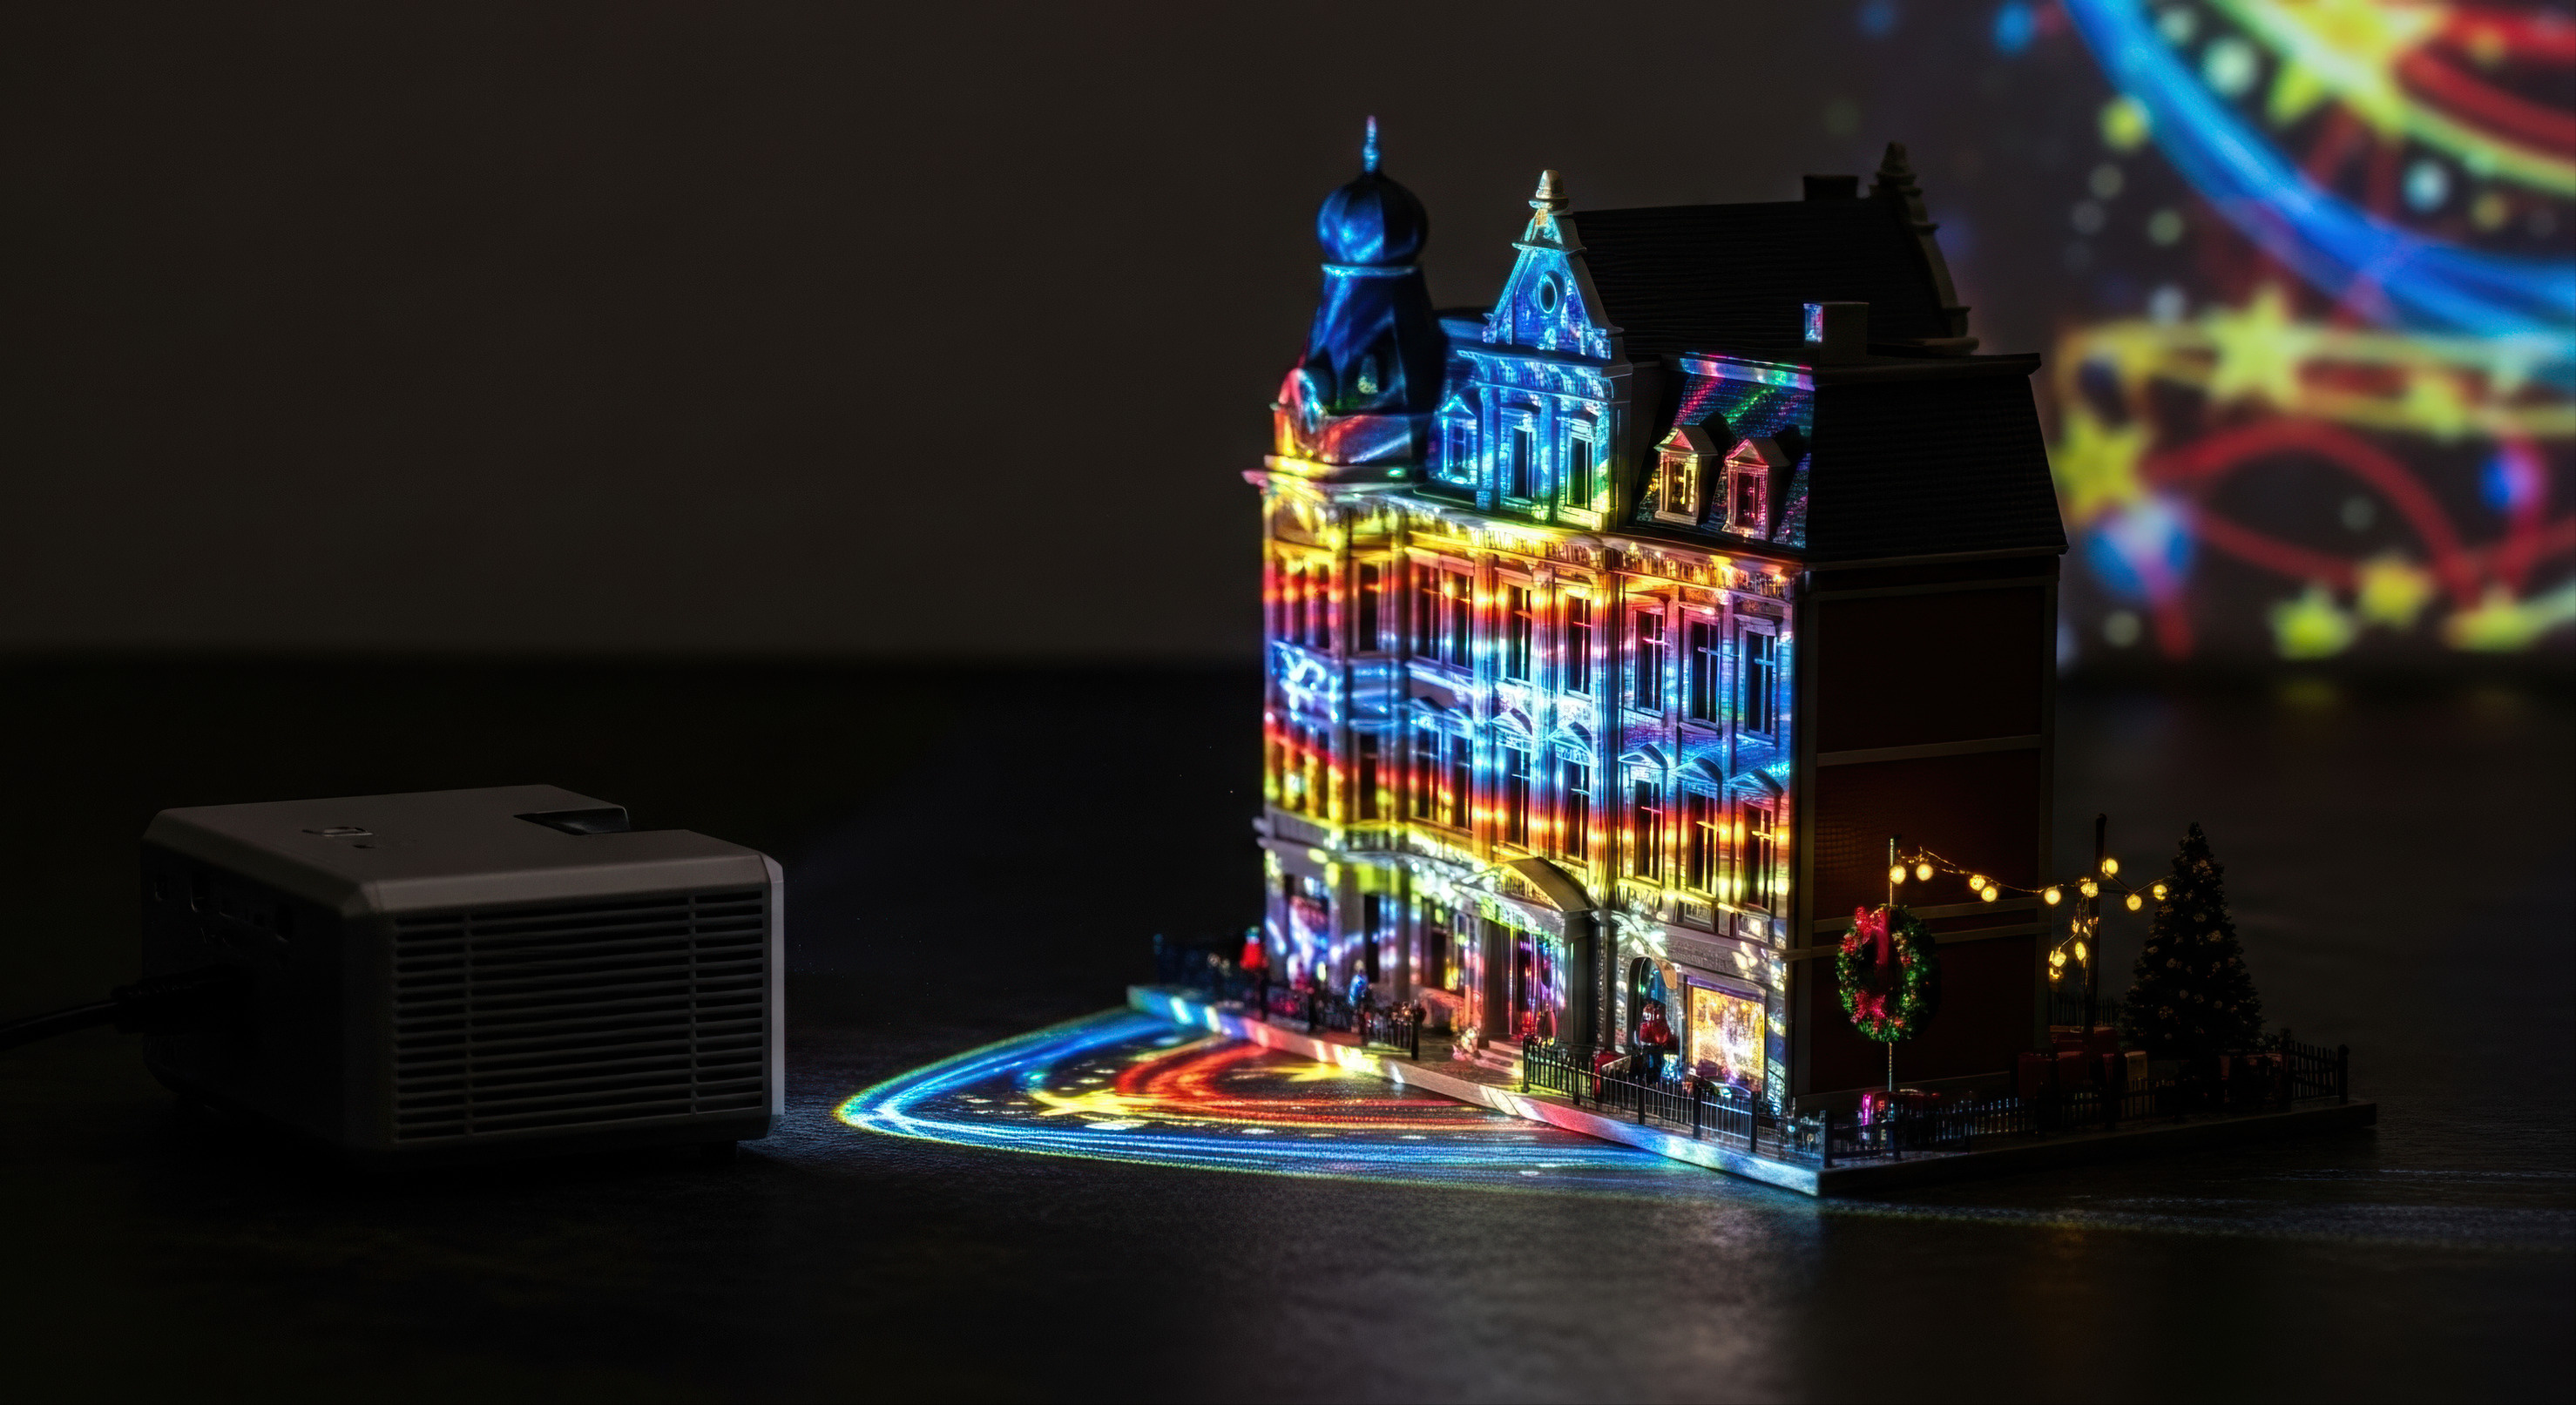
\includegraphics[width=0.5\linewidth]{thesis/figures/sample.jpeg}
    \caption{図の基本的な載せ方}
    \label{fig:basic}
\end{figure}

\verb|figure|環境の配置オプションは，希望する位置を\LaTeX に伝えるものである（表\ref{tab:floatpos}）．
複数指定すると上から順に試される．基本は\verb|[htbp]|か\verb|[tb]|でよい．

\begin{table}[htbp]
    \centering
    \caption{フロートの配置オプション}
    \label{tab:floatpos}
    \begin{tabular}{cl}\toprule
        記号 & 意味 \\ \midrule
        \texttt{h} & その場（here）に置く \\
        \texttt{t} & ページ上部（top） \\
        \texttt{b} & ページ下部（bottom） \\
        \texttt{p} & 図表専用ページ（page） \\
        \texttt{H} & 強制的にその場（\texttt{here}パッケージ） \\ \bottomrule
    \end{tabular}
\end{table}

%% ===========================================================
\section{画像サイズの指定}
\label{sec:imgsize}
\verb|\includegraphics|のオプションで，画像の大きさを複数の方法で指定できる．

\begin{description}[leftmargin=*, style=nextline]
    \item[幅で指定] \verb|[width=0.8\linewidth]|：本文幅の80\%にする（最もよく使う）．
    \item[高さで指定] \verb|[height=4cm]|：高さを4cmにする．
    \item[倍率で指定] \verb|[scale=0.5]|：元の大きさの0.5倍にする．
    \item[縦横比を保つ] \verb|[width=5cm,height=3cm,keepaspectratio]|：指定範囲に収め，比率は保つ．
\end{description}

幅の基準には，本文幅を表す\verb|\linewidth|（\verb|\textwidth|）のほか，
段組み時の段幅\verb|\columnwidth|が使える．比率で指定しておくと，
レイアウトが変わっても自動で追従するため便利である．

%% ===========================================================
\section{画像の回転とトリミング}
\label{sec:imgtrim}
\verb|angle|で画像を回転でき，\verb|trim|と\verb|clip|で周囲を切り取れる（図\ref{fig:rotate}，\ref{fig:trim}）．

\begin{figure}[htbp]
    \centering
    \begin{minipage}[b]{0.45\linewidth}
        \centering
        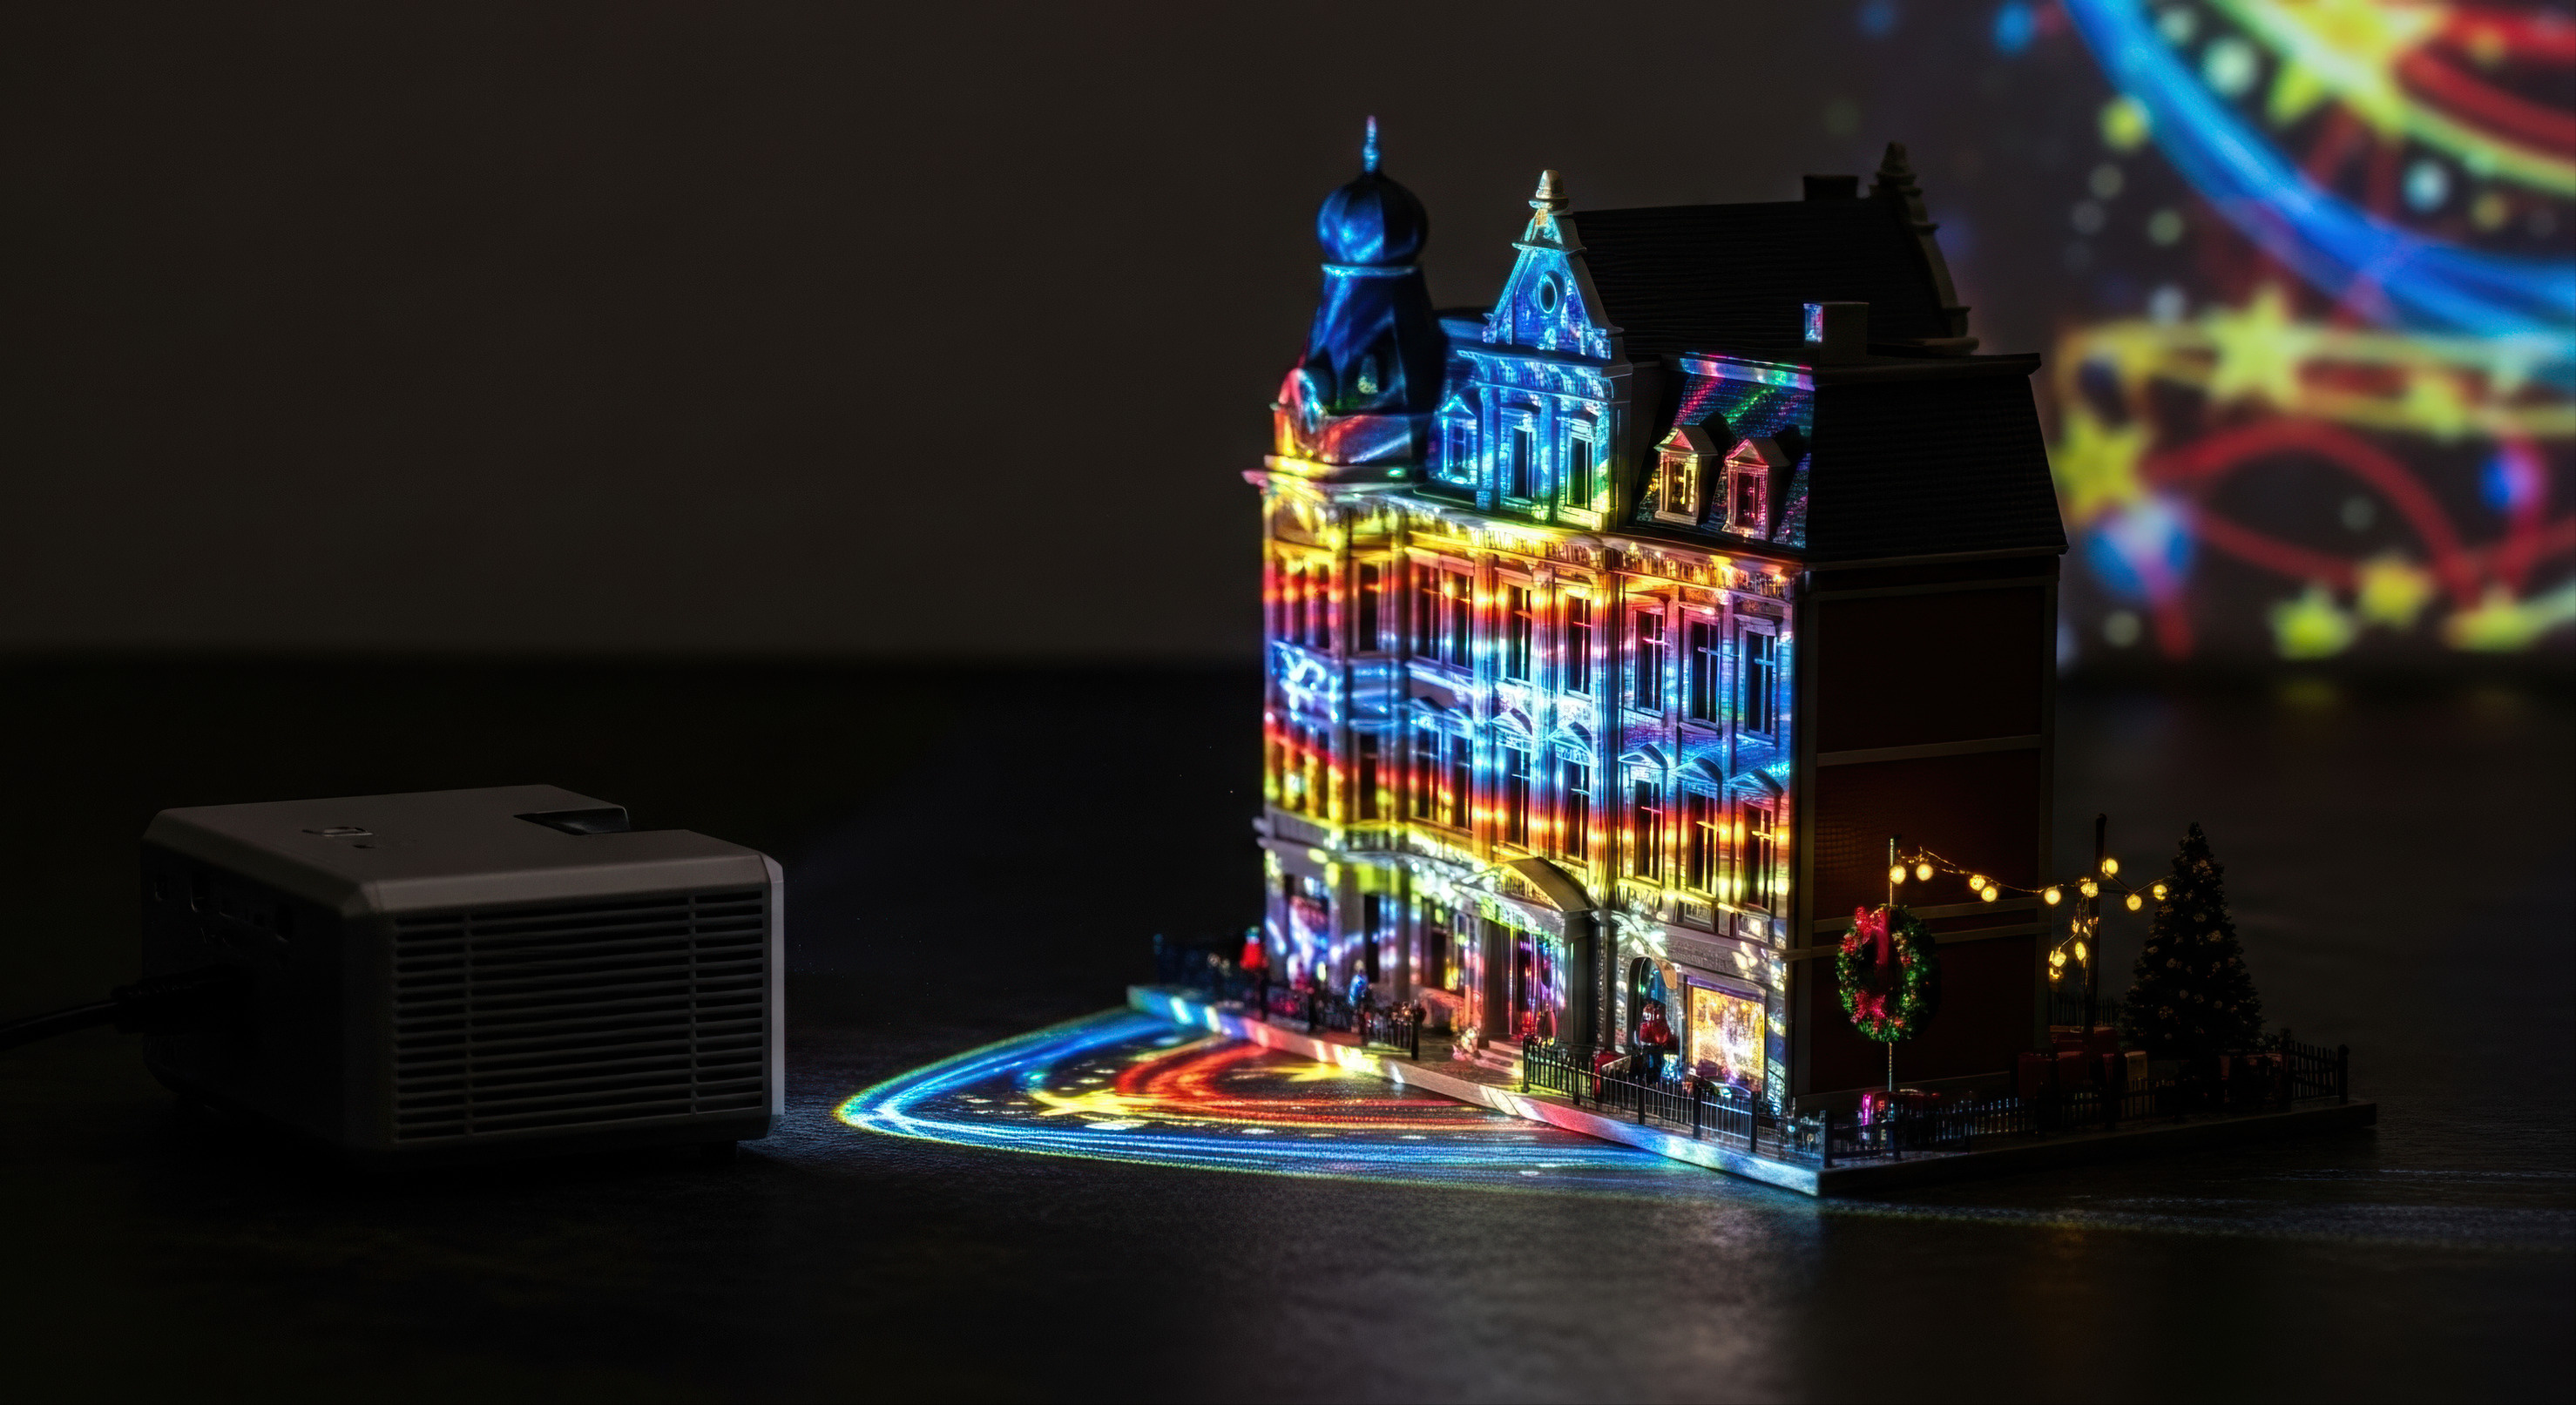
\includegraphics[width=0.5\linewidth, angle=90]{thesis/figures/sample.jpeg}
        \caption{\texttt{angle=90}で90度回転}
        \label{fig:rotate}
    \end{minipage}\hfill
    \begin{minipage}[b]{0.45\linewidth}
        \centering
        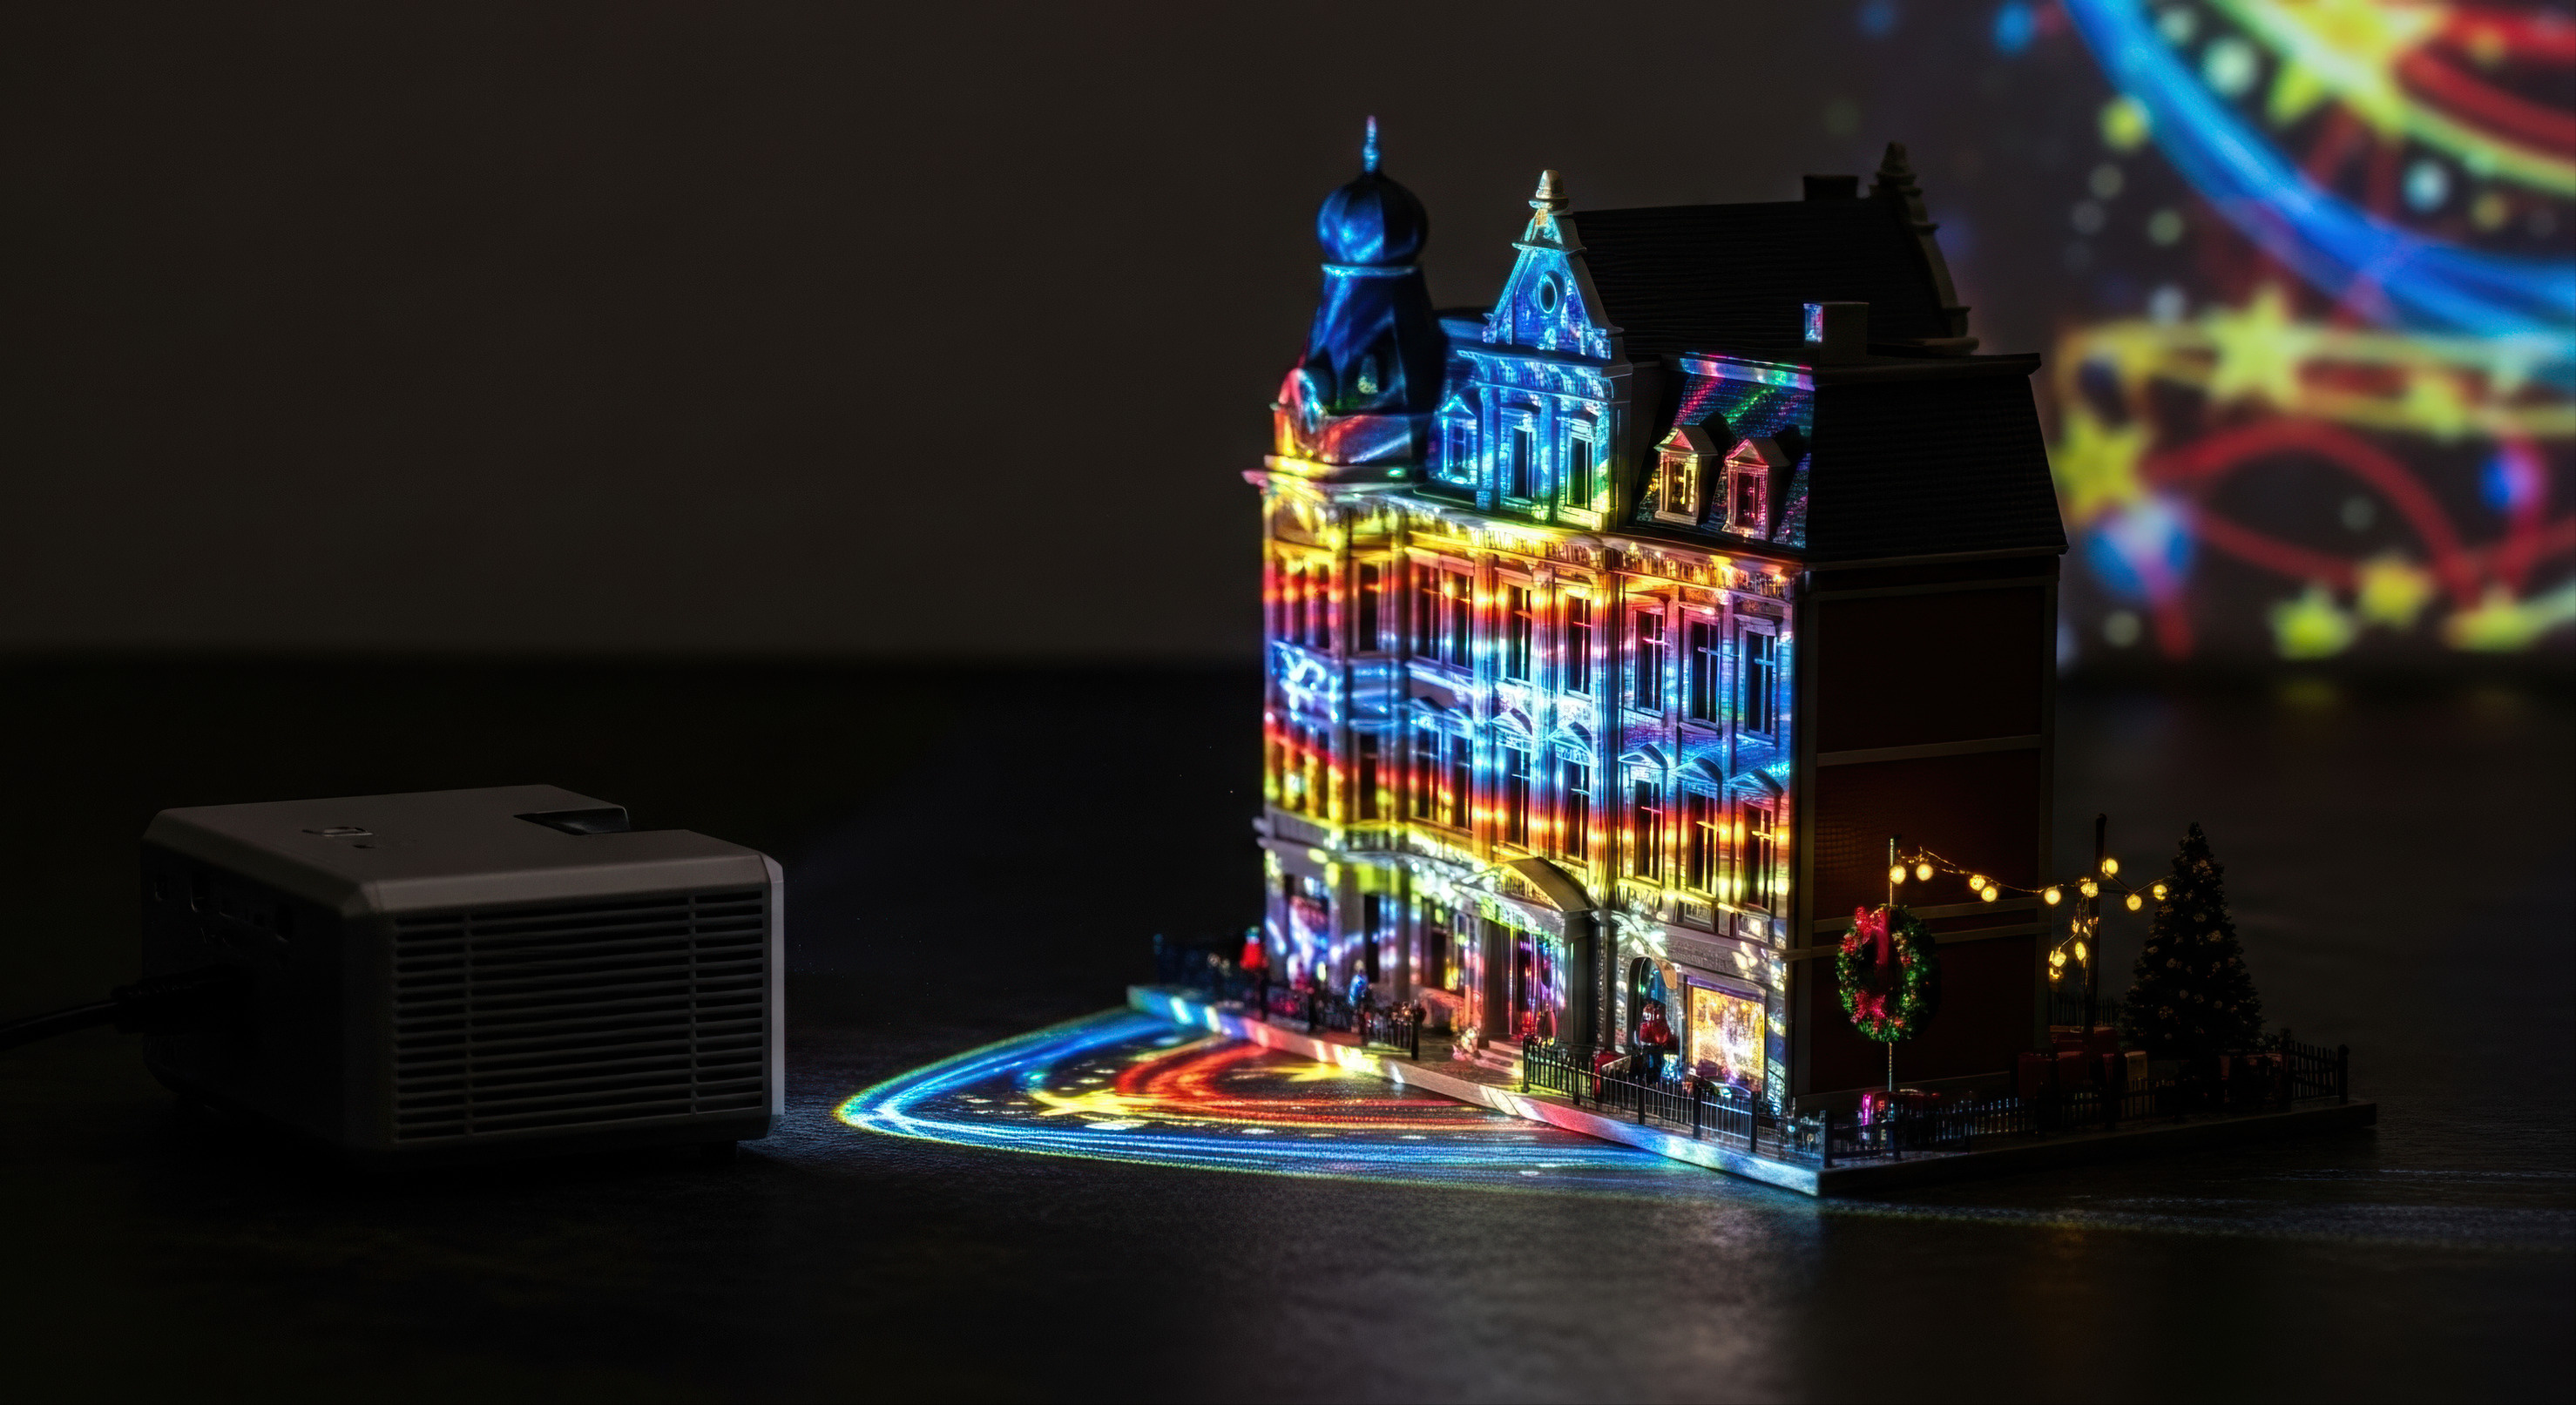
\includegraphics[width=0.6\linewidth, trim=200 200 200 200, clip]{thesis/figures/sample.jpeg}
        \caption{\texttt{trim+clip}で周囲を切り取り}
        \label{fig:trim}
    \end{minipage}
\end{figure}

\verb|trim=左 下 右 上|の順に切り取る量を指定し，\verb|clip|を付けると指定範囲外が表示されなくなる．

%% ===========================================================
\section{図を横に並べる}
\label{sec:sidebyside}
図を横に並べる方法は2通りある．キャプションを1つにまとめるか，個別に付けるかで使い分ける．

1つ目は\texttt{minipage}で並べる方法で，図\ref{fig:rotate}と図\ref{fig:trim}がその例である（個別キャプション）．
2つ目は\texttt{subcaption}で，1つの図番号の下に (a)(b)(c) と枝番号を付ける方法である（図\ref{fig:subs}）．

\begin{figure}[htbp]
    \centering
    \begin{subfigure}[b]{0.3\linewidth}
        \centering
        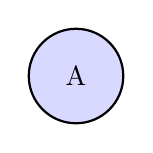
\begin{tikzpicture}\draw[thick,fill=blue!15](0,0)circle(0.6);\node at(0,0){A};\end{tikzpicture}
        \subcaption{円}\label{fig:sub-a}
    \end{subfigure}\hfill
    \begin{subfigure}[b]{0.3\linewidth}
        \centering
        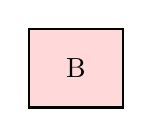
\begin{tikzpicture}\draw[thick,fill=red!15](0,0)rectangle(1.2,1.0);\node at(0.6,0.5){B};\end{tikzpicture}
        \subcaption{四角形}\label{fig:sub-b}
    \end{subfigure}\hfill
    \begin{subfigure}[b]{0.3\linewidth}
        \centering
        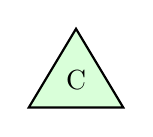
\begin{tikzpicture}\draw[thick,fill=green!15](0,0)--(1.2,0)--(0.6,1.0)--cycle;\node at(0.6,0.35){C};\end{tikzpicture}
        \subcaption{三角形}\label{fig:sub-c}
    \end{subfigure}
    \caption{subcaptionで枝番号を付けた例（図\subref{fig:sub-a}〜\subref{fig:sub-c}）}
    \label{fig:subs}
\end{figure}

%% ===========================================================
\section{本文を図に回り込ませる}
\label{sec:wrap}
\texttt{wrapfig}の\texttt{wrapfigure}環境を使うと，図の横に本文を回り込ませられる．
小さな図でページを節約したいときに有効である．

\begin{wrapfigure}{r}{0.32\linewidth}
    \centering
    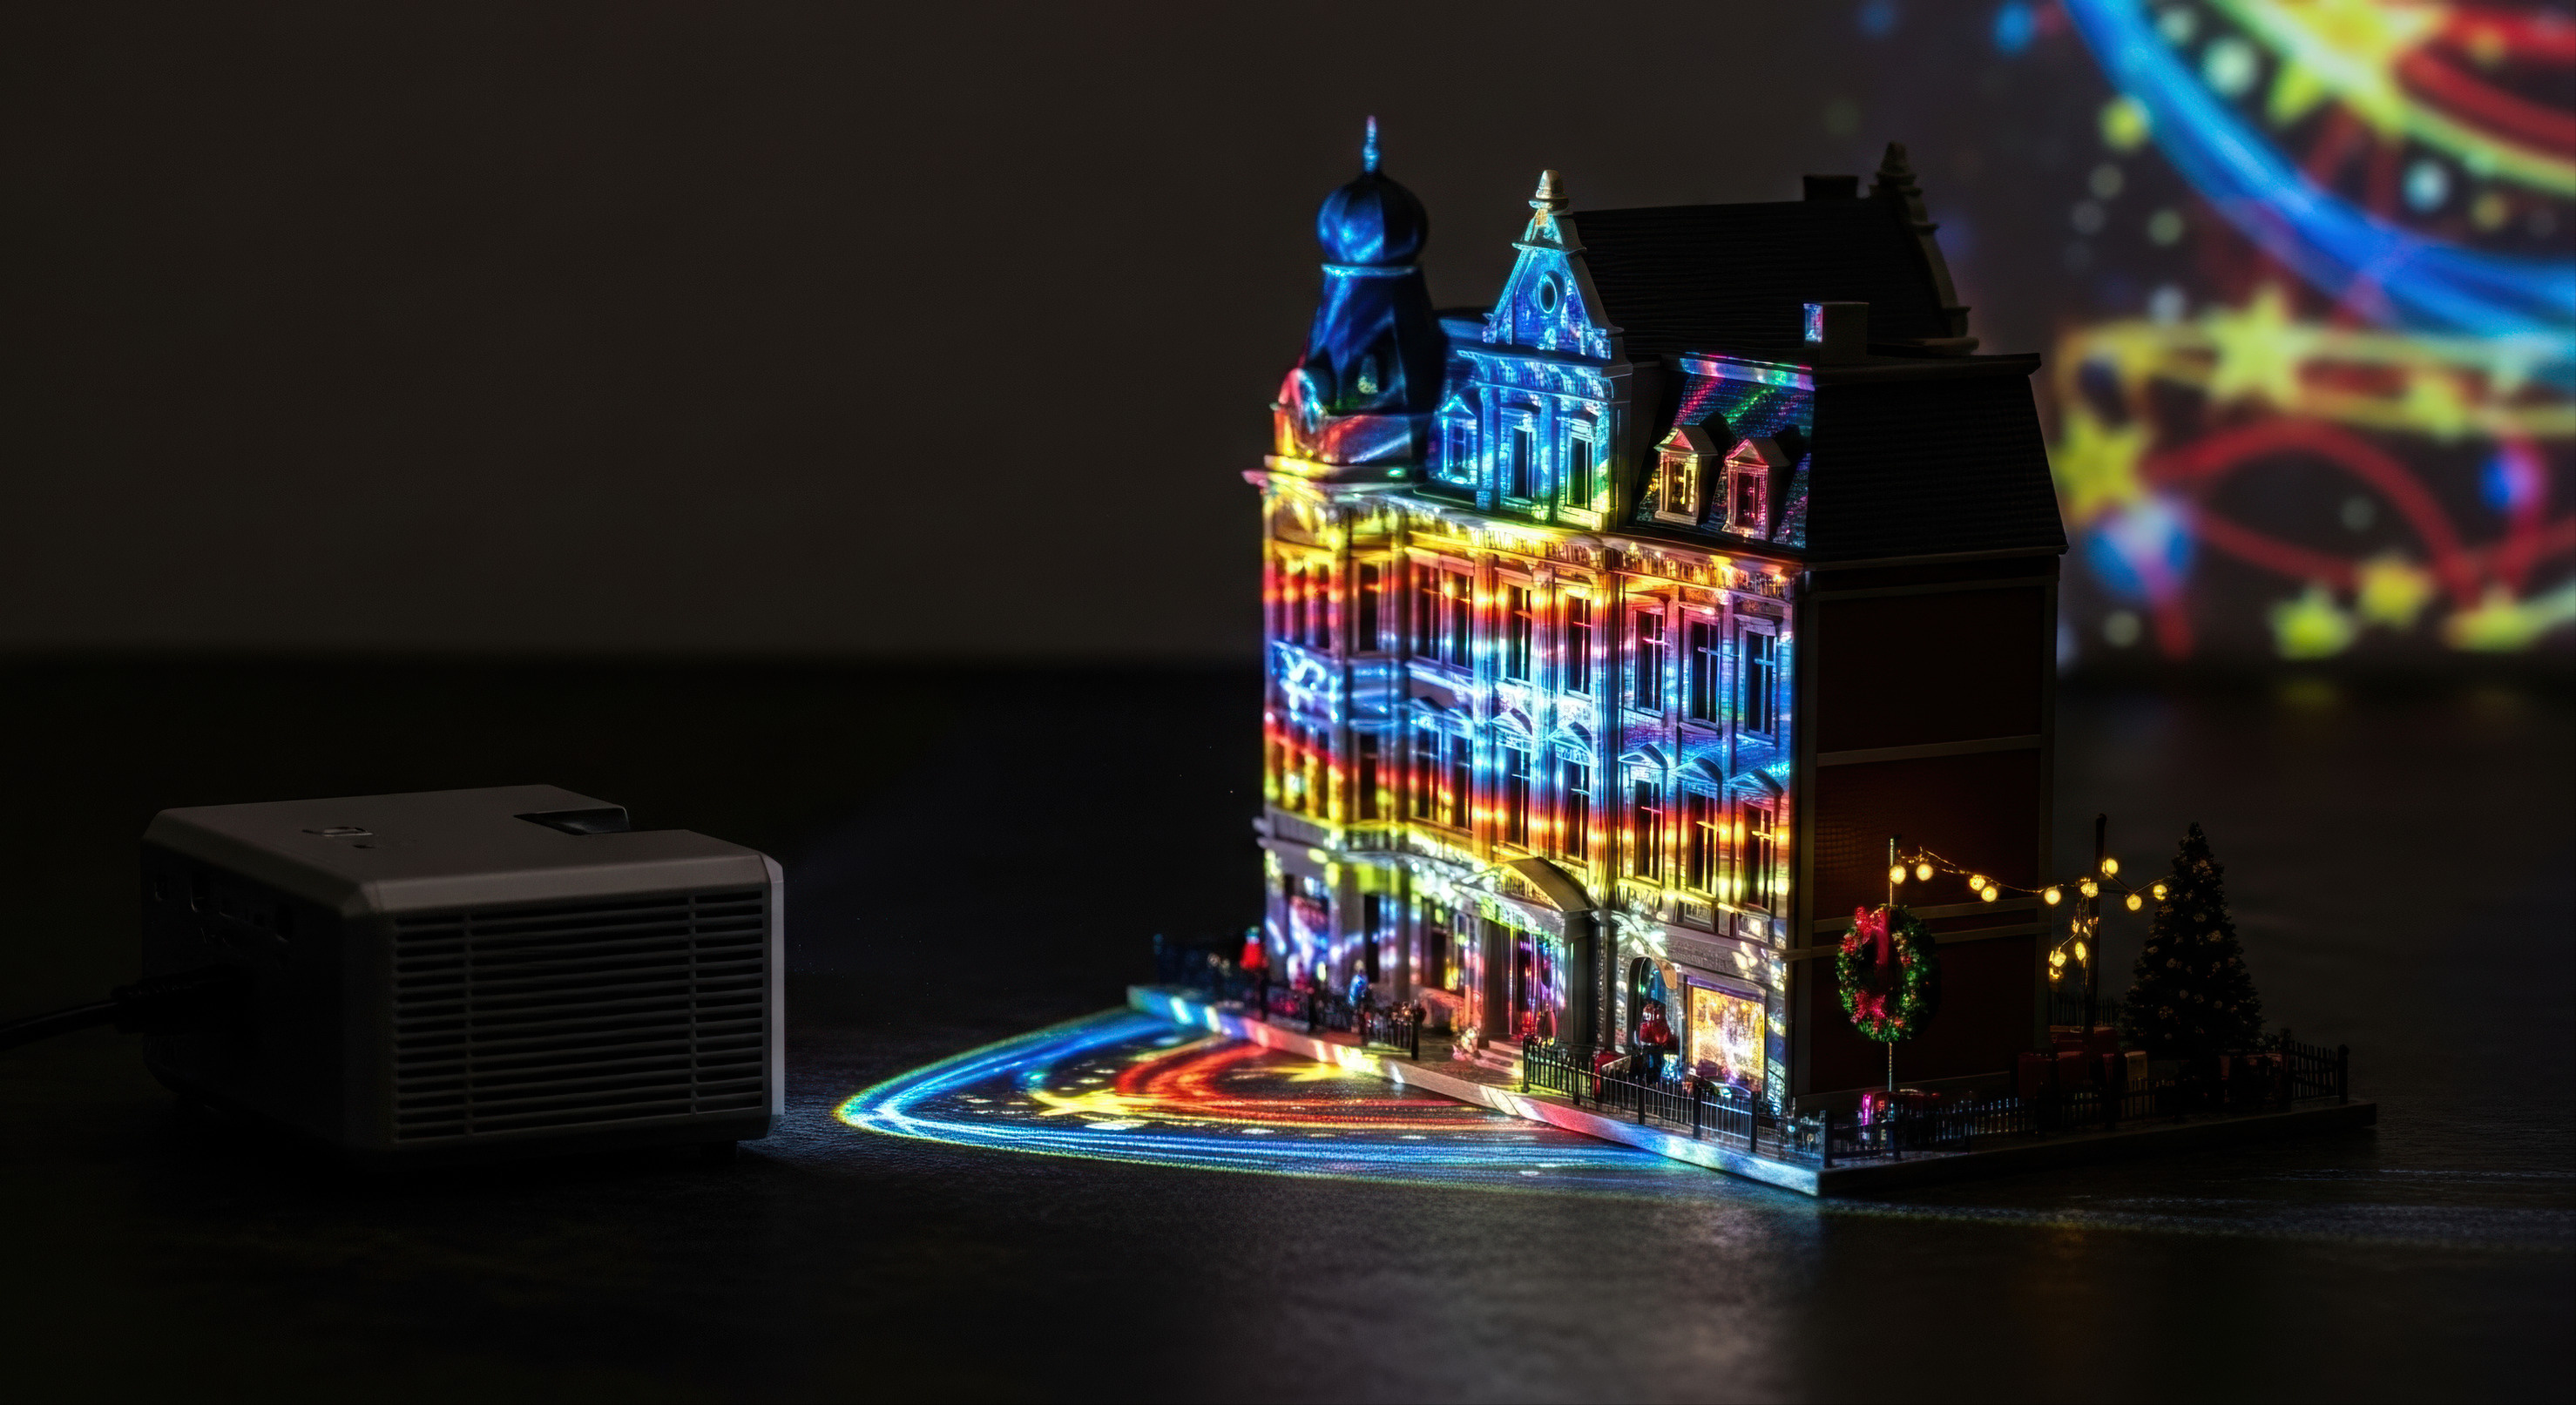
\includegraphics[width=0.9\linewidth]{thesis/figures/sample.jpeg}
    \caption{回り込みの例}
    \label{fig:wrap}
\end{wrapfigure}
\verb|\begin{wrapfigure}{r}{0.32\linewidth}|のように，第1引数で図を置く側（\texttt{r}：右，\texttt{l}：左），
第2引数で図の幅を指定する．図\ref{fig:wrap}のように，本文が図の脇に回り込んで配置される．
ただし回り込みは前後のレイアウトが乱れやすいため，使いどころには注意し，
段落の先頭付近に置くと安定しやすい．本文が十分にあると，このように自然に回り込む．
回り込ませる図はあまり大きくしすぎないことが，きれいに仕上げるこつである．

%% ===========================================================
\section{TikZ で図を描く}
\label{sec:tikz}
\texttt{TikZ}を使うと，\LaTeX 内でベクター形式の図を直接描ける．
拡大しても劣化せず，フォントも本文と統一できる（図\ref{fig:tikz}）．

\begin{figure}[htbp]
    \centering
    \begin{tikzpicture}[
        node distance=2cm,
        block/.style={draw, rounded corners, minimum width=1.8cm, minimum height=0.9cm},
        every edge/.style={draw, -{Stealth}, thick}]
        \node[block, fill=blue!10]  (in)   {入力};
        \node[block, fill=orange!15, right=of in]   (proc) {処理};
        \node[block, fill=green!10,  right=of proc] (out)  {出力};
        \draw (in) edge (proc) (proc) edge (out);
    \end{tikzpicture}
    \caption{TikZによるフロー図}
    \label{fig:tikz}
\end{figure}

%% ===========================================================
\section{pgfplots でグラフを描く}
\label{sec:pgfplots}
\texttt{pgfplots}を使うと，数値データから直接グラフを描ける（図\ref{fig:plot}）．
外部の画像を貼るより，体裁を本文と統一できる利点がある．

\begin{figure}[htbp]
    \centering
    \begin{tikzpicture}
        \begin{axis}[
            width=0.7\linewidth, height=5cm,
            xlabel={エポック}, ylabel={精度},
            legend pos=south east, grid=major]
            \addplot coordinates {(1,0.62)(2,0.74)(3,0.81)(4,0.86)(5,0.90)};
            \addlegendentry{提案手法}
            \addplot coordinates {(1,0.58)(2,0.66)(3,0.71)(4,0.75)(5,0.78)};
            \addlegendentry{従来手法}
        \end{axis}
    \end{tikzpicture}
    \caption{pgfplotsによる折れ線グラフ}
    \label{fig:plot}
\end{figure}

%% ===========================================================
\section{横向きページの大きな図表}
\label{sec:landscape}
縦幅に収まらない大きな図表は，\texttt{lscape}の\texttt{landscape}環境で
ページを横向きにすると収まりやすい（表\ref{tab:landscape}）．

\begin{landscape}
    \begin{table}[htbp]
        \centering
        \caption{横向きページに配置した表の例}
        \label{tab:landscape}
        \begin{tabular}{lcccccc}\toprule
            条件 & 指標1 & 指標2 & 指標3 & 指標4 & 指標5 & 指標6 \\ \midrule
            設定A & 0.81 & 0.79 & 0.85 & 0.88 & 0.90 & 0.77 \\
            設定B & 0.83 & 0.82 & 0.86 & 0.84 & 0.91 & 0.80 \\ \bottomrule
        \end{tabular}
    \end{table}
\end{landscape}

%% ===========================================================
\section{表の基本}
\label{sec:table}
表は\texttt{table}環境に入れ，キャプションは表の上に付ける（表\ref{tab:basic}）．
中身は\texttt{tabular}環境で組み，列指定で各列の揃え方を決める
（\texttt{l}：左揃え，\texttt{c}：中央，\texttt{r}：右揃え）．
\texttt{booktabs}の\verb|\toprule|・\verb|\midrule|・\verb|\bottomrule|で罫線を引く．
一般的な表では縦罫線を使わない方が読みやすい．

\begin{table}[htbp]
    \centering
    \caption{基本的な表}
    \label{tab:basic}
    \begin{tabular}{lcr}\toprule
        項目（左） & 区分（中央） & 値（右） \\ \midrule
        りんご & A & 120 \\
        みかん & B & 80 \\ \bottomrule
    \end{tabular}
\end{table}

%% ===========================================================
\section{セルの結合と部分罫線}
\label{sec:cellmerge}
\verb|\multicolumn|で列方向，\verb|\multirow|で行方向にセルを結合できる．
\verb|\cmidrule|を使うと，一部の列にだけ罫線を引ける（表\ref{tab:merge}）．

\begin{table}[htbp]
    \centering
    \caption{セル結合と部分罫線の例}
    \label{tab:merge}
    \begin{tabular}{lccc}\toprule
        \multirow{2}{*}{手法} & \multicolumn{2}{c}{評価指標} & \multirow{2}{*}{時間 [ms]} \\
        \cmidrule(lr){2-3}
                & 精度 [\%] & F1値 & \\ \midrule
        手法A    & 85.2 & 0.83 & 120 \\
        手法B    & 91.7 & 0.90 & 340 \\
        提案手法  & \textbf{93.4} & \textbf{0.92} & 150 \\ \bottomrule
    \end{tabular}
\end{table}

%% ===========================================================
\section{幅の制御・数値揃え・色付き表}
\label{sec:tablewidth}
\texttt{tabularx}を使うと，表全体の幅を指定し，\texttt{X}列に残り幅を自動配分できる．
長い文を含むセルは自動で折り返される（表\ref{tab:tabularx}）．

\begin{table}[htbp]
    \centering
    \caption{tabularxで幅を指定した表}
    \label{tab:tabularx}
    \begin{tabularx}{\linewidth}{lX}\toprule
        項目 & 説明 \\ \midrule
        概要 & \texttt{X}列は残りの幅を自動的に占め，長い文章でも指定幅で折り返される． \\
        補足 & 列指定の\texttt{p\{3cm\}}でも，幅を固定して折り返せる． \\ \bottomrule
    \end{tabularx}
\end{table}

数値を小数点で揃えたい場合は\texttt{siunitx}の\texttt{S}列が便利である．
また\texttt{colortbl}の\verb|\rowcolor|で行に色を付けられる（表\ref{tab:num}）．

\begin{table}[htbp]
    \centering
    \caption{数値揃え（S列）と行の色付け}
    \label{tab:num}
    \begin{tabular}{l S[table-format=3.2]}\toprule
        項目 & {測定値} \\ \midrule
        \rowcolor{blue!8}
        測定1 & 12.30 \\
        測定2 & 105.07 \\
        測定3 & 7.50 \\ \bottomrule
    \end{tabular}
\end{table}

%% ===========================================================
\section{ページをまたぐ表}
\label{sec:longtable}
行数が多くページをまたぐ表には\texttt{longtable}を用いる．
\verb|\endhead|で各ページに繰り返す見出し行を指定できる．

\begin{longtable}{cl}
    \caption{longtableによる長い表}\label{tab:long}\\
    \toprule 番号 & 内容 \\ \midrule
    \endfirsthead
    \toprule 番号 & 内容（続き） \\ \midrule
    \endhead
    \bottomrule
    \endfoot
    1 & 1行目 \\
    2 & 2行目 \\
    3 & 3行目 \\
\end{longtable}

%% ===========================================================
\section{数式}
\label{sec:math}
文中の数式は\verb|$...$|で囲む（例：$y = ax + b$）．
独立した別行立ての数式は，番号が不要なら\verb|\[ ... \]|，
番号を付けて参照するなら\texttt{equation}環境を用いる（式(\ref{eq:softmax})）．

\begin{equation}
    \label{eq:softmax}
    \mathrm{softmax}(z_i) = \frac{e^{z_i}}{\sum_{j=1}^{K} e^{z_j}}
\end{equation}

複数行で等号位置を揃えるには\texttt{align}を，番号を付けず並べるだけなら\texttt{gather}を用いる．

\begin{align}
    f(x) &= (x+1)^2 \notag \\
         &= x^2 + 2x + 1
\end{align}

場合分けには\texttt{cases}，行列には\texttt{pmatrix}（丸括弧）や\texttt{bmatrix}（角括弧）を使う．
括弧の大きさは\verb|\left|・\verb|\right|で中身に自動で合わせられる．

\begin{equation}
    \mathrm{sgn}(x) =
    \begin{cases}
        \ 1  & (x > 0) \\
        \ 0  & (x = 0) \\
        -1   & (x < 0)
    \end{cases}
    \qquad
    A = \left( \begin{matrix} a & b \\ c & d \end{matrix} \right)
\end{equation}

総和$\sum_{i=1}^{n}$，積分$\int_a^b f(x)\,dx$，極限$\lim_{n\to\infty}$，
分数$\frac{1}{2}$，平方根$\sqrt{x}$，ギリシャ文字（$\alpha, \beta, \gamma, \pi$），
上付き$x^2$・下付き$x_i$など，多くの記号が\texttt{amsmath}・\texttt{amssymb}で利用できる．
数式中で日本語や立体の語を書くには\verb|\text{...}|や\verb|\mathrm{...}|を用いる．
数式中の変数や記号は，本文中で必ずその意味を説明すること．

%% ===========================================================
\section{定義・定理環境}
\label{sec:theorem}
定義や定理は専用の環境で記述でき，章ごとに自動で採番される．

\begin{definition}[エントロピー]
    確率分布 $p = (p_1, \dots, p_n)$ のエントロピー $H(p)$ を次式で定義する．
    \begin{equation}
        H(p) = -\sum_{i=1}^{n} p_i \log p_i
    \end{equation}
\end{definition}

\begin{theorem}
    台が有限な確率分布の中で，一様分布はエントロピーを最大にする．
\end{theorem}
\begin{proof}
    Lagrangeの未定乗数法により示せる（詳細は省略する）．
\end{proof}

%% ===========================================================
\section{ソースコード}
\label{sec:code}
ソースコードは\texttt{listings}の\texttt{lstlisting}環境で掲載する（ソースコード\ref{lst:fib}）．
\verb|caption|・\verb|label|でキャプションと参照を，\verb|language|で言語を指定すると，
キーワードや文字列に自動で色が付く．論文の主張に関係する部分のみを抜粋すること．

\begin{lstlisting}[caption={Pythonによる例}, label={lst:fib}, language=Python, float=tb]
# フィボナッチ数列の第 n 項を返す関数
def fib(n):
    a, b = 0, 1
    for _ in range(n):
        a, b = b, a + b
    return a
\end{lstlisting}

文中に短いコードを埋め込むには\verb|\verb|や\verb|\texttt{}|を用いる（例：\verb|print(x)|）．
外部ファイルをそのまま読み込んで掲載するには\verb|\lstinputlisting|を用いる．

\begin{lstlisting}[language={[LaTeX]TeX}, numbers=none, frame=single]
\lstinputlisting[language=Python]{src/main.py}
\end{lstlisting}

%% ===========================================================
\section{アルゴリズム}
\label{sec:algorithm}
擬似コードは\texttt{algorithm}（フロート）と\texttt{algpseudocode}（擬似コード本体）で記述する（アルゴリズム\ref{alg:bsearch}）．

\begin{algorithm}[htbp]
    \caption{二分探索}
    \label{alg:bsearch}
    \begin{algorithmic}[1]
        \Require ソート済み配列 $A[1..n]$，探索値 $x$
        \Ensure $x$ の添字（存在しなければ $-1$）
        \State $lo \gets 1,\quad hi \gets n$
        \While{$lo \le hi$}
            \State $mid \gets \lfloor (lo + hi) / 2 \rfloor$
            \If{$A[mid] = x$}
                \State \Return $mid$
            \ElsIf{$A[mid] < x$}
                \State $lo \gets mid + 1$
            \Else
                \State $hi \gets mid - 1$
            \EndIf
        \EndWhile
        \State \Return $-1$
    \end{algorithmic}
\end{algorithm}

%% ===========================================================
\section{枠囲みと外部PDFの挿入}
\label{sec:box}
注意点やまとめは枠で囲むと目立つ．\texttt{ascmac}の\texttt{itembox}を用いた例を示す．

\begin{itembox}[l]{提出前チェックリスト}
    \begin{itemize}
        \item \verb|\ThisIsDraft|を削除したか
        \item 図表・参考文献に未参照・未定義がないか
        \item overfull が発生していないか（第\ref{sec:overfull}節参照）
    \end{itemize}
\end{itembox}

既存のPDF（アンケート用紙やデータシートなど）を付録として丸ごと挿入するには，
\texttt{pdfpages}の\verb|\includepdf|を用いる．

\begin{lstlisting}[language={[LaTeX]TeX}, numbers=none, frame=single]
\includepdf[pages=-]{appendix/questionnaire.pdf} % 全ページ挿入
\end{lstlisting}

%% ===========================================================
\section{Overfullへの対処}
\label{sec:overfull}
組版時に行が右側にはみ出す現象を overfull という．原則として overfull を起こさないよう工夫する．
発生しやすい例として，長い英単語・URL・数式・\verb|\verb|コマンドがある．
URLは\verb|\url{}|で囲む，長い英単語は適切な位置で改行を許可するなどの対処を行う．
\verb|\\|や\verb|\linebreak|による強制改行での回避はできるだけ避ける．
